% Created 2017-10-23 Mon 13:26
\documentclass{article}
\usepackage[utf8]{inputenc}
\usepackage[T1]{fontenc}
\usepackage{fixltx2e}
\usepackage{graphicx}
\usepackage{longtable}
\usepackage{float}
\usepackage{wrapfig}
\usepackage{rotating}
\usepackage[normalem]{ulem}
\usepackage{amsmath}
\usepackage{textcomp}
\usepackage{marvosym}
\usepackage{wasysym}
\usepackage{amssymb}
\usepackage{hyperref}
\tolerance=1000
\usepackage{tabularx,graphicx,ragged2e,booktabs,caption,float}
\usepackage[margin=0.8in]{geometry}
\usepackage{amsmath}
\usepackage{gensymb}
\usepackage{authblk}
\setlength{\parskip}{0.2cm}
\setlength{\parindent}{0.85cm}
\author{Tiankai Xiong}
\date{\today}
\title{PC5215, Lab2}
\hypersetup{
  pdfkeywords={},
  pdfsubject={},
  pdfcreator={Emacs 25.3.1 (Org mode 8.2.10)}}
\begin{document}

\maketitle

\section{Question 1}
\label{sec-1}

The results are presented in Figure \ref{fig:Q1}

\begin{figure}[H]
  \centering
  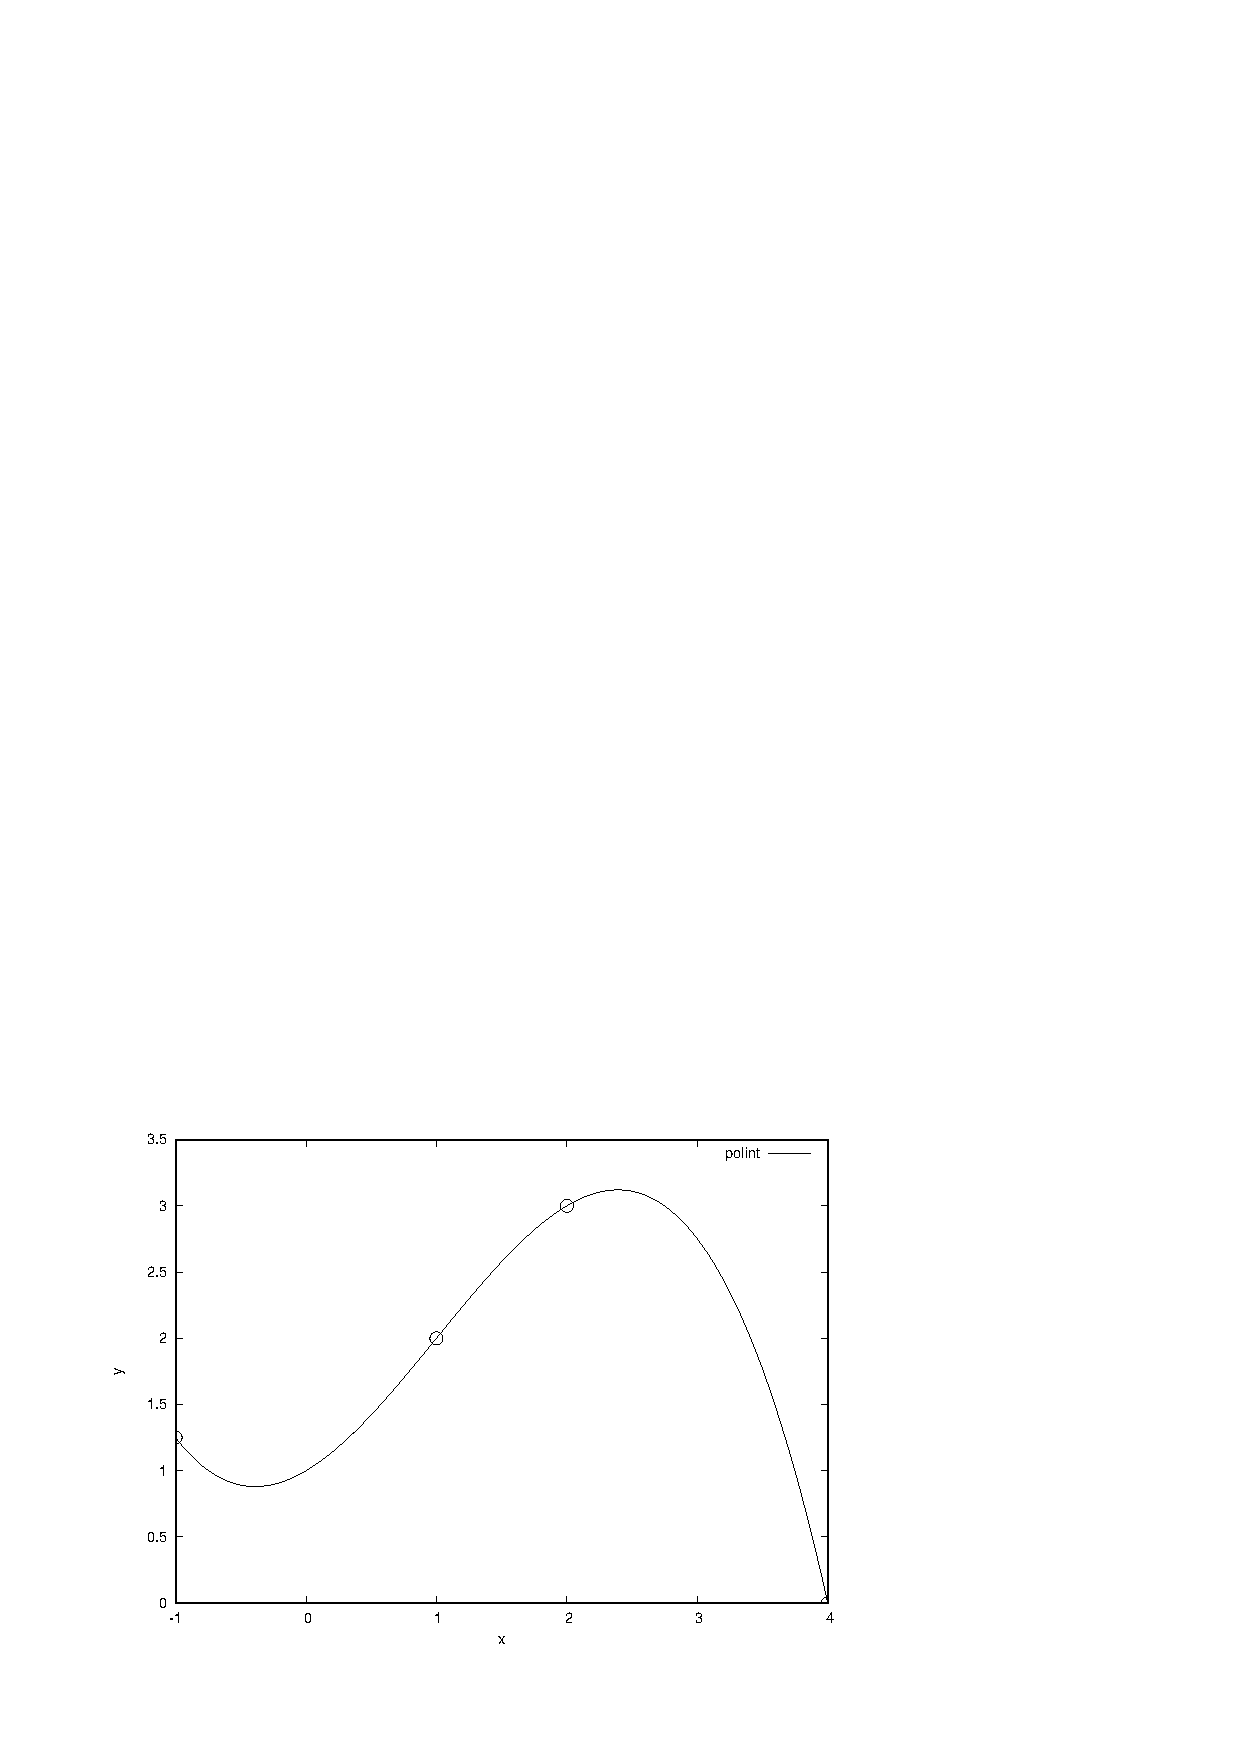
\includegraphics[width=0.6\textwidth]{Q1.pdf}
  \caption{Interpolation by polint}
  \label{fig:Q1}
\end{figure}

\section{Question 2}
\label{sec-2}

Since the effect of using high precision is trivial, so is that of
$\epsilon$, we only test combinations of K and JMAX(Otherwise the
number of combinations will be huge). Here we always use double
precision, and let $EPS = 1.0^{-20}$

\begin{longtable}{|c|c|c|c|c|}
\caption{\label{tbl:Q2}Result and discrepancy with different K and JMAX}
\\
\hline
K & JMAX & double & discrepancy\\
\hline
\endhead
\hline\multicolumn{4}{r}{Continued on next page} \\
\endfoot
\endlastfoot
1 & 10 & 23.098167602860964819910805090331 & 14.944803483049799552873082575388\\
5 & 10 & 0.000000000000000000000000000000 & -8.153364119811165267037722514942\\
10 & 10 & 8.153364119811161714324043714441 & -0.000000000000003552713678800501\\
20 & 10 & 0.000000000000000000000000000000 & -8.153364119811165267037722514942\\
50 & 10 & 0.000000000000000000000000000000 & -8.153364119811165267037722514942\\
\hline
1 & 20 & 23.098167602860964819910805090331 & 14.944803483049799552873082575388\\
5 & 20 & 0.000000000000000000000000000000 & -8.153364119811165267037722514942\\
10 & 20 & 8.153364119811161714324043714441 & -0.000000000000003552713678800501\\
20 & 20 & 8.153364119811136845328292110935 & -0.000000000000028421709430404007\\
50 & 20 & 0.000000000000000000000000000000 & -8.153364119811165267037722514942\\
\hline
1 & 30 & 23.098167602860964819910805090331 & 14.944803483049799552873082575388\\
5 & 30 & 0.000000000000000000000000000000 & -8.153364119811165267037722514942\\
10 & 30 & 8.153364119811161714324043714441 & -0.000000000000003552713678800501\\
20 & 30 & 8.153364119811136845328292110935 & -0.000000000000028421709430404007\\
50 & 30 & 0.000000000000000000000000000000 & -8.153364119811165267037722514942\\
\hline
\end{longtable}

From Table \ref{tbl:Q2}, we can interpret that
\begin{enumerate}
\item At low values of K, the integral is very inaccurate. Clearly, if
we only use one point to extrapolate, the result has very little chance to be accurate.
\item Only a range of K give promising results.
\item The value of JMAX does not matter as long as it's not too small.
\end{enumerate}

It is hard to explain why only a range of K give promising
results. It might be an error when we implemented the functions with
index starting from 0.

The most accurate result obtained is presented in Figure \ref{fig:Q2}

\begin{figure}[H]
  \centering
  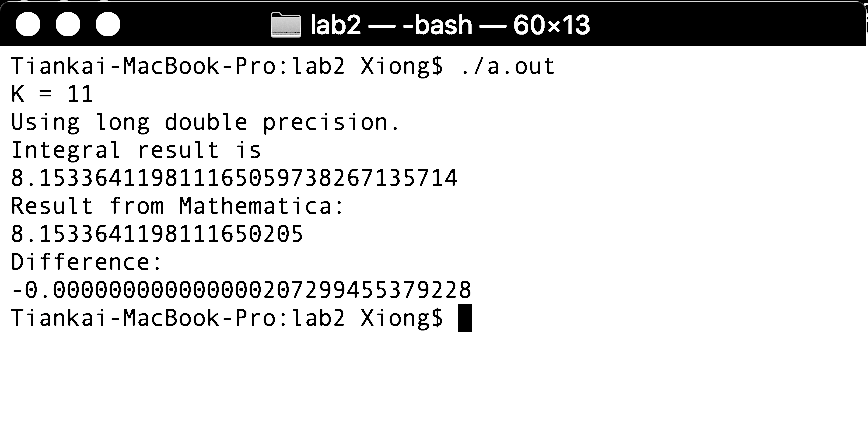
\includegraphics[width=0.6\textwidth]{Q2_best_result.png}
  \caption{Best result obtained}
  \label{fig:Q2}
\end{figure}

\section{Question 2}
\label{sec-3}
\subsection{Method}
\label{sec-3-1}

The Hamiltonian, which is provided in SI units, can be re-written
in atomic units:

\begin{equation}
  \hat{H} = -\frac{1}{2}\nabla^2_1 - \frac{1}{2}\nabla^2_2 - \frac{1}{r_{A1}}
  - \frac{1}{r_{B1}}  - \frac{1}{r_{A2}}  - \frac{1}{r_{B2}}  + \frac{1}{r_{12}}
   + \frac{1}{r_{AB}}
\end{equation}

With the wave function given as:

\begin{equation}
  \Psi(\vec{r_1}, \vec{r_2} = \phi(r_{A1}) \phi(r_{B2}) + \phi(r_{A2}) \phi(r_{B1})), \quad \phi(r) = e^{-r/a_0}
\end{equation}

We can calculate $\Psi \hat{H} \Psi$ on Mathematica which gives:

\begin{equation}
  \Psi (e^{-r_{A2} - r_{B1}}(-1 + \frac{1}{r_{a2}} + \frac{1}{r_{b1}}) + e^{-r_{a1} - r_{b2}}(-1 + \frac{1}{r_{a1}} + \frac{1}{r_{b2}}) +
  (-\frac{1}{r_{a1}} -\frac{1}{r_{b1}} -\frac{1}{r_{a2}} -\frac{1}{r_{b2}} +\frac{1}{r_{12}}  +\frac{1}{r_{ab}}  )*\psi)
\end{equation}

Where no conjugation is needed because the wave function and operators have only real components.

To find the total energy at given $r_{AB}$, we use MC Metropolis
algorithm. The probability of a combination of $\vec{r_1},
   \vec{r_2}$, $P(\vec{r_1}, \vec{r_2})$ can be calculated by $\Psi
   \Psi$. Despite not normalized, it does not affect the implementation of Metropolis algorithm.

The logic is as follows: at each step, we choose a random set of
$(\vec{r_1}, \vec{r_2})$ based on previous positions, and compare
$P_n$ the previous probability density and $P_{n+1}$ the current
probability density. If $P_{n+1} > P_n$, we accept the new
configuration, and calculate ∑

Each time we have a new pair of $\Psi \hat{H} \Psi$, we add them to
the existing values of each, followed by updating the value of total energy by:

\begin{equation}
  E =\frac{ \sum\Psi \hat{H} \Psi}{\sum\Psi \Psi }
\end{equation}

When two values of $E$ differ smaller than a preset $\epsilon$, the loop terminates and we record a pair of $(r_{AB}, E)$.
\subsection{Results}
\label{sec-3-2}

The plot of the pair $(r_{AB}, E)$ is presented in Figure
\ref{fig:rE}. It is observed that the minimum energy is achieved at
around $r_{AB} = 1a_0$, and the total energy is about $-1.4
   \,\text{Hartree}$. Putting accuracy aside, the shape of the graph
presents a typical relation between energy and bond length where
the energy reaches a minimum at some points near Bohr radius. The
total energy approaches zero when the distance reaches infinity.


\begin{figure}[H]
  \centering
  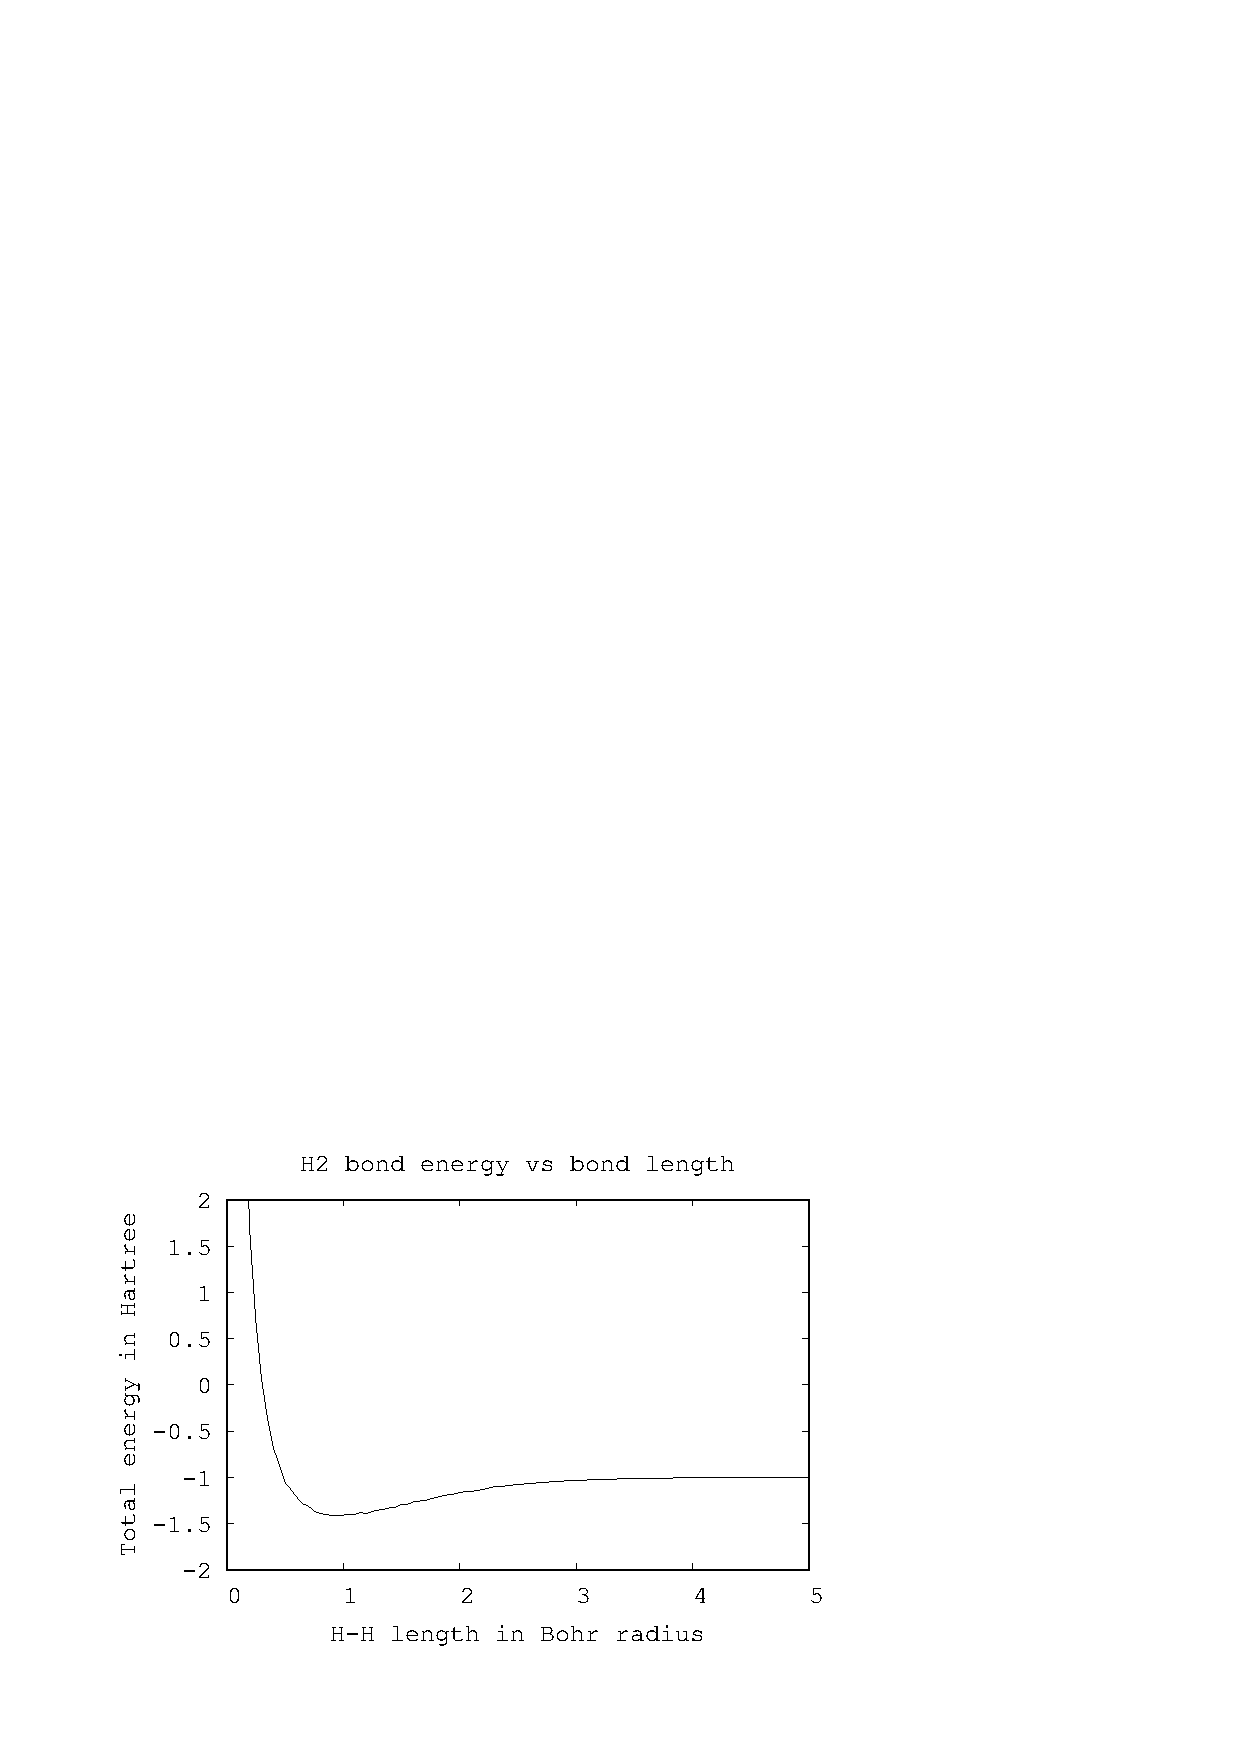
\includegraphics[width=0.8\textwidth]{Q3.pdf}
  \caption{Plot of total energy against distance between two atoms}
  \label{fig:rE}
\end{figure}

To illustrate, we have selected data at $r_{AB} = 0.5 a_0, \;
   r_{AB} = 1.0 a_0, \; r_{AB} = 8.0 a_0$ to plot the electron
cloud (Figure \ref{fig:0.5}, \ref{fig:1.0}, \ref{fig:8.0}). Clearly,
after a certain distance, electrons of the two protons will not
migrate to the other proton, thus giving us a configuration of two
separate hydrogen atoms.


\begin{figure}[H]
  \centering
  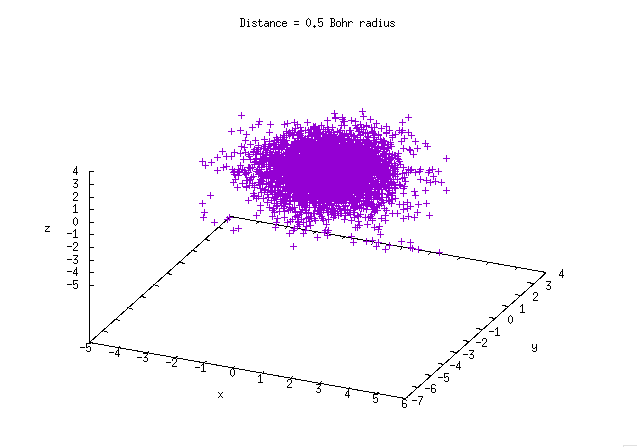
\includegraphics[width=0.6\textwidth]{05.png}
  \caption{Electron cloud at r = 0.5 Bohr radius}
  \label{fig:0.5}
\end{figure}

\begin{figure}[H]
  \centering
  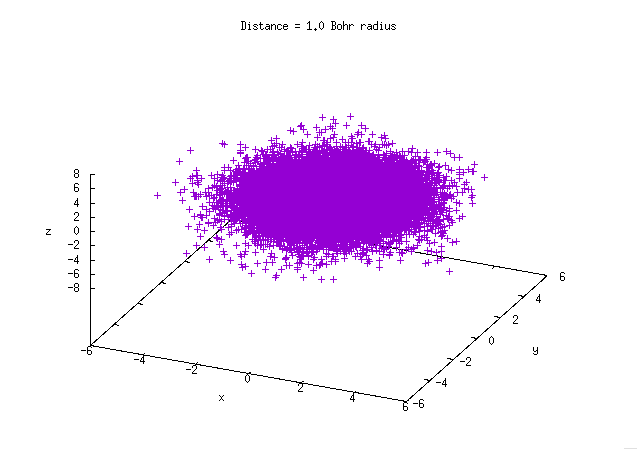
\includegraphics[width=0.6\textwidth]{10.png}
  \caption{Electron cloud at r = 1.0 Bohr radius}
  \label{fig:1.0}
\end{figure}

\begin{figure}[H]
  \centering
  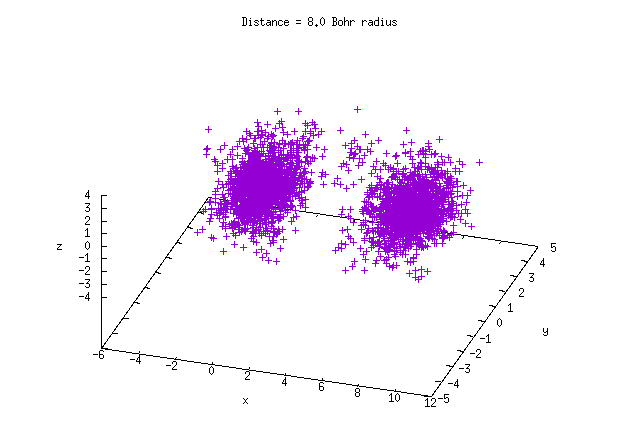
\includegraphics[width=0.6\textwidth]{80.png}
  \caption{Electron cloud at r = 8.0 Bohr radius}
  \label{fig:8.0}
\end{figure}

\section{SRC}
\label{sec-4}

\begin{itemize}
\item \texttt{lab2\_1.c}
\end{itemize}
\hline
\begin{verbatim}
#include <stdio.h>
#include <stdlib.h>
#include <math.h>
#include "lab2.h"


int main(){

  // The function polint() is written in the fashion that the index
  // starts from 0
  double xa[4] = {-1.0, 1.0, 2.0, 4.0};
  double ya[4] = {1.25, 2.0, 3.0, 0.0};

  int n = 4;

  double *y = (double *)malloc(sizeof(double));
  double *dy = (double *)malloc(sizeof(double));

  FILE *fp;

  fp = fopen("Q1.dat", "w+");
  for(double x = -1.0; x<=4.0; x+=0.01){

    polint(xa, ya, n, x, y, dy);
    fprintf(fp, "%f  %f\n", x, *y);

  }
  fclose(fp);

  return(0);


}
\end{verbatim}

\hline

\begin{itemize}
\item \texttt{lab2\_2.c}
\end{itemize}
\hline
\begin{verbatim}
#include <stdio.h>
#include "lab2.h"


double _function(double x){
  return (pow(x, 4) * log(x + sqrt(pow(x, 2) +1)));
};

int main(){

  double integral = qromb(_function, 0.0, 2.0);
  printf("K = %d\n", K);
  printf("Using double precision.\n");
  printf("Integral result is \n%.30f\n", integral);
  printf("Result from Mathematica: \n8.1533641198111650205\n");
  printf("Difference: \n%.30f\n", integral - 8.1533641198111650205);

}
\end{verbatim}

\hline

\begin{itemize}
\item \texttt{lab2\_3.c}
\end{itemize}
\hline
\begin{verbatim}
#include <stdio.h>
#include <time.h>
#include <stdlib.h>
#include <math.h>

#define EPS 1.0e-10
#define STEP 1.0e-2

void randomR(double *r){

  double dx = ((double)rand()/RAND_MAX - 0.5)*2;
  double dy = ((double)rand()/RAND_MAX - 0.5)*2;
  double dz = ((double)rand()/RAND_MAX - 0.5)*2;



  // in the rare case where r = (0, 0, 0) will be obtained, redo
  if(r[0] == -dx && r[1] == -dy && r[2] == -dz){
    randomR(r);
    printf("This actually happend!\n");
  }

  r[0] += dx;
  r[1] += dy;
  r[2] += dz;


};

void updateR(double *r){
  r[3] = r[0];
  r[4] = r[1];
  r[5] = r[2];

};

void resetR(double *r){
  r[0] = r[3];
  r[1] = r[4];
  r[2] = r[5];
}

double norm(double *u, double *v, int n){

  double result = 0.0;
  for(int i = 0; i< n; i++){
    result += pow((u[i]-v[i]), 2);
  }
  return sqrt(result);
};


double psi(double *r1, double *r2, double *rA, double *rB){

  double psiA1 = exp(-norm(rA, r1, 3));
  double psiB2 = exp(-norm(rB, r2, 3));
  double psiA2 = exp(-norm(rA, r2, 3));
  double psiB1 = exp(-norm(rB, r1, 3));

  double psi = psiA1*psiB2 + psiA2*psiB1;

  return psi;

};

double php(double *r1, double *r2, double *rA, double *rB){
  double PHP = 0.0;
  double P = psi(r1, r2, rA, rB);
  double K, V;                  /* Kinetic and potential */

  // result copied from mathematica
  K = exp(-norm(r2, rA, 3) - norm(r1, rB, 3))*(-1 + 1/(norm(r2, rA, 3)) + 1/norm(r1, rB, 3))+
    exp(-norm(r1, rA, 3) - norm(r2, rB, 3))*(-1 + 1/norm(r1, rA, 3) + 1/norm(r2, rB, 3)    );



  V = (-1/norm(rA, r1, 3) - 1/norm(rB, r1, 3) - 1/norm(rA, r2, 3) - 1/norm(rB, r2, 3)
       +1/norm(r1, r2, 3) + 1/norm(rA, rB, 3))*P;


  double HP = K + V;

  PHP = P*HP;
  return PHP;
};


int main(){

  srand(time(NULL));            /* seed the RNG */
  // r1 and r2 will store the current position and there previous positions
  double r1[6];
  double r2[6];


  double rA[3] = {0.0, 0.0, 0.0}; /* fix A at origin */
  double rB[3] = {0.0, 0.0, 0.0}; /* w/o loss of generality fix B
                                         on the x-axis */

  double p1, p2;                /* previous P(r1, r2) and current P(r1, r2) */

  double PHP;                /* \psi H \psi */
  double PP;                 /* \psi \psi */



  double Energy1,  Energy2;

  FILE *OUTPUT_FILE;
  OUTPUT_FILE = fopen("Q3.dat", "w+");
  int counter;


  for(int i = 5; i*STEP < 10; ++i){
    PHP = 0.0;
    PP = 0.0;
    r1[0] = i*STEP/2; r1[1] = 0.0; r1[2] = 0.0; /* initiate the electrons between the two nuclei */
    r2[0] = i*STEP/2; r2[1] = 0.0; r2[2] = 0.0;
    randomR(r1); randomR(r2);     /* generate random r1, r2 */
    updateR(r1); updateR(r2);     /* update data */
    rB[0] = i*STEP;
    counter = 0;
    Energy1 = -0.1;             /* reset energies */
    Energy2 = 0.0;

    p1 = pow(psi(r1, r2, rA, rB), 2);    /* initiate p1 */


    FILE *RECORD_FILE;
    if(i*STEP == 0.5){
      RECORD_FILE = fopen("0.5.dat", "w+");
    }else if(i*STEP == 1.0){
      RECORD_FILE = fopen("1.0.dat", "w+");
    }else if(i*STEP == 8.0){
      RECORD_FILE = fopen("8.0.dat", "w+");
    }

    do{


      randomR(r1);                /* generate random r1 */
      randomR(r2);                /* and r2 */
      p2 = pow(psi(r1, r2, rA, rB), 2); /* calculate new proba */

      if(p2 > p1 || p2/p1 > (double)rand()/RAND_MAX){
        Energy1 = Energy2;
        /* if this case if more likely, or it is taken with a pabability p2/p1 */
        updateR(r1); updateR(r2); /* update the positions */
        p1 = p2;                  /* and probability */
        PHP += php(r1, r2, rA, rB);
        PP += p2;                 /* add the value to PP */
        counter++;
        Energy2 = PHP/PP;

        if(i*STEP ==0.5||i*STEP == 1.0 || i*STEP == 8.0){
          fprintf(RECORD_FILE, "%f %f %f\n", r1[0], r1[1], r1[2]);
          fprintf(RECORD_FILE, "%f %f %f\n", r2[0], r2[1], r2[2]);

        }


      }else{
        resetR(r1); resetR(r2);
      }




    }while(fabs(Energy1-Energy2) >= EPS);
    if(RECORD_FILE) fclose(RECORD_FILE);
    printf("%d steps for i= %d\n", counter, i);

    fprintf(OUTPUT_FILE, "%f  %f\n", i*STEP, Energy2);
  }
  fclose(OUTPUT_FILE);




}
\end{verbatim}

\hline

\begin{itemize}
\item \texttt{lab2.h}
\end{itemize}
\hline
\begin{verbatim}
#include <stdio.h>
#include <stdlib.h>
#include <math.h>


#define EPS 1.0e-20
#define JMAX 10
#define JMAXP (JMAX+1)
#define K 1

#define FUNC(x) ((*func)(x))


void polint(double xa[], double ya[], int n, double x, double *y, double *dy){

  int i, m, ns = 0;
  double den, dif, dift, ho, hp, w;
  double *c, *d;

  dif = fabs(x - xa[0]);
  c = (double *)malloc(n * sizeof(double));
  d = (double *)malloc(n * sizeof(double));

  for(i = 0; i < n; i++){       /* Here we find the index ns of the
                                   closest table entry */
    if((dift = fabs(x-xa[i])) < dif){
      ns = i;
      dif = dift;
    }
    c[i] = ya[i];               /* and initialize the tableau of c's
                                   and d's */
    d[i] = ya[i];
    /* This should return c and d as xa and ya, if n = dim(xa) */
  }
  *y = ya[ns--];                /* This is the initial approximation
                                   to y */
  for(m =1; m<n; m++){
    for(i = 0; i< n-m; i++){
      ho = xa[i]-x;
      hp = xa[i+m] -x;
      w = c[i+1] - d[i];
      if((den = ho-hp) == 0.0) printf("Error in routine polint\n");
      /* This error can occur only if two input xa'a are(to within
         roundoff) identical */
      den = w/den;
      d[i] = hp*den;            /* Here the c's and d's are updated */
      c[i] = ho*den;
    }
    *y += (*dy = (2*(ns + 1 ) < (n-m) ? c[ns + 1] : d[ns--]));
    /* After each column in the tableau is completed, we decide which
       correction, c or d, we want to add to our accumulating value of
       y. i.e. which path to take through the tableau--forking up or
       down. We do this in such a way as to take the most "straight
       line" route through the tableau to its apex, updating ns
       accordingly to keep track of where we are. This route keeps the
       partial approximations centered(insofar as possible) on the
       target x. The last dy added is thus the error indication. */
  }
  free(d);
  free(c);


};

double trapzd(double (*func)(double), double a, double b, int n){
  double x, tnm, sum, del;
  static double s;
  int it, j;

  if(n == 1){
    return (s = 0.5*(b-a)*(FUNC(a)+FUNC(b)));
  }else{
    for (it = 1, j = 1; j < n -1; j++){
      it <<= 1;
    }
    tnm = it;
    del = (b-a)/tnm;
    x = a + 0.5*del;
    for(sum = 0.0, j = 0; j<it; j++, x+=del){
      sum += FUNC(x);
    }
    s = 0.5*(s+(b-a)*sum/tnm);
    return s;

  }

};




double qromb(double (*func)(double), double a, double b){


  void polint(double xa[], double ya[], int n, double x, double *y, double *dy);
  double trapzd(double (*func)(double), double a, double b, int n);
  double ss, dss;
  double s[JMAX], h[JMAXP];
  int j;

  h[0] = 1.0;
  for (j = 1; j<=JMAX; j++){
    s[j-1] = trapzd(func, a, b, j-1);
    if (j >= K){
      polint(&h[j-K], &s[j-K], K, 0.0, &ss, &dss);
      if(fabs(dss) <= EPS*fabs(ss)){
        return ss;
      }
    }
    h[j] = 0.25*h[j-1];
  }
  printf("Too many steps in routine qromb\n");
  return 0.0;
};
\end{verbatim}

\hline
% Emacs 25.3.1 (Org mode 8.2.10)
\end{document}
